% !Mode:: "TeX:UTF-8"
\chapter{emscripten结构剖析}

\section{emscripten的文件结构}

emscripten有几个关键组件:

\begin{itemize}
    \item {\heiti clang:}llvm的编译器前端,c/c++/objc语言的解释器,用来生成llvm字节码;
    \item {\heiti emscripten:}llvm的编译器后端,用来将中间代码 (llvm bytecode,扩展名为.bc)编译成符合asm.js标准的\upcite{herman2013asm}js文件;
    \item {\heiti node:}Node.js的核心是Google V8引擎。Google V8引擎的一个著名的Javascript运行环境(runtime)。借助Node.js,可以在命令行下直接测试执行JavaScript代码;
    \item {\heiti spidermonkey(可选):}Mozilla开发的用C语言实现的JavaScript脚本引擎;
    \item {\heiti crunch(可选):}一个实时的DXT贴图压缩和实时转码工具。
\end{itemize}

\subsection{clang的目录结构}

代码\ref{clang-directory-structure}(具体在附录A中)是clang的文件结构,其中,e1.35.0\_64bit文件夹代表我使用的emscripten版本号为1.35.0,64位版。

受限于篇幅限制,只介绍几个重要命令。
bugpoint命令用来给程序打断点,用于调试。
clang以及clang开头的一些命令,则是文件编译命令,用来把代码源文件转换为llvm字节码。
llc命令用来将纯文本格式的中间代码 (llvm-IR文件) 编译成纯文本格式 (非二进制格式) 的本地汇编代码。
lli命令用来解释llvm\text{-}IR文件,即用来解释llvm的字节码。
llvm\text{-}as命令用来将文本格式的llvm IR编译成二进制 llvm IR。
llvm\text{-}dis命令是反汇编命令,可以把二进制 llvm IR 转换成文本格式 llvm IR,功能和llvm\text{-}as正好相反。
llvm\text{-}objdump可以导出内存信息,用于调试。
optimizer命令用来优化程序。

\subsection{emscripten的目录结构}

代码\ref{emscripten-directory-structure}是emscripten的目录结构。

cmake文件夹下存储了几个模块。主要用于解决openAL和openGL程序移植时的依赖问题。
docs文件夹下是Alon Zakai先生的论文\upcite{zakai2011emscripten},讲解了emscripten的一些原理以及性能分析。
emcc/em++对应gcc中的gcc/g++,是c和c++的编译命令。
emcmake对应linux系统工具cmake,可以在使用CMakeLists.txt文件时快速替换系统编译命令为emscripten内部命令。
emmake对应linux自带的构建工具make,可以在使用Makefile文件作为项目配置文件时,使用emscripten内部命令替换默认编译命令,缺点是依赖问题不好解决。
site文件夹用来存放emscripten的相关文档。
src文件夹下保存了一些常用的类库转换后的js文件,在编译后加入生成后的js文件中,比如library\_glut.js和library\_openal.js文件,都是运行时需要的文件。
system文件夹中存储了一些常用类库的头文件和lib文件,用来在编译时使用。原作者Alon Zakai也是一个游戏开发爱好者,为了openGL和openAL以及SDL程序等多媒体的移植,在emscripten中内置了GL,GLUT,GLEW,GLFW,GLES,SDL,openAL等多他特别优化过的多媒体库。
tests文件夹下是一些emscripten的测试用例。
third\_party文件夹下存放了一些插件和第三方工具,其中的WebIDL可以用来调整语言接口,实现C++和js代码的相互调用。
tools文件夹下存放了一些实用工具,比如用来调试编译后的js文件的工具,混合js文件的工具和优化js文件的工具。


\subsection{node.js命令解析}

node.js只提供两个命令。
node命令用来执行一个js文件。
npm则是node.js的包管理命令,类似ruby的gem已经python的pip命令,用来进行在线的包管理已经本地项目管理。

\section{emscripten编译c/c++文件操作}

emscripten的核心命令为emcc,类似gcc的gcc命令\upcite{li1990catch},用来快速的编译、链接某个c/c++文件。
下面以hello world程序为例。

\subsection{“Hello world”程序源代码}

代码\ref{c-hello-world-sample}即为一个简单示例。

\begin{lstlisting}[
    language={C},
    caption={Hello World程序的源代码},
    label={c-hello-world-sample},
]
#include <stdio.h>

int main()
{
    printf("Hello, world!");
    return 0;
}
\end{lstlisting}

\subsection{“Hello world”程序源移植过程}

下面的命令\ref{bash-hello-world-sample}可以完成c/c++代码向JavaScript的转换。

\begin{lstlisting}[
    language={bash},
    caption={Hello World程序的源代码编译命令},
    label={bash-hello-world-sample},
]

# 生成一个名为a.out.js的JavaScript文件,可以被JavaScript虚拟机执行
emcc hello.c

# 生成一个网页,可以直接查看效果
emcc hello.c -o hello_world.html
\end{lstlisting}

\subsection{“Hello world”程序运行效果}

图\ref{hello-world-sample-cli}展示了移植程序在命令行下运行的效果。

\begin{figure}[h!] % [h!] 表示尽量排在当前位置
    \centering
    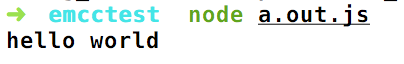
\includegraphics[width=200bp]{figure/pic/hello-world-sample-cli.png}
    \caption{hello world移植程序在cli(node.js)下运行效果}
    \label{hello-world-sample-cli}
\end{figure}

图\ref{hello-world-sample-html}展示了移植程序在浏览器中运行的效果。

\begin{figure}[h!] % [h!] 表示尽量排在当前位置
    \centering
    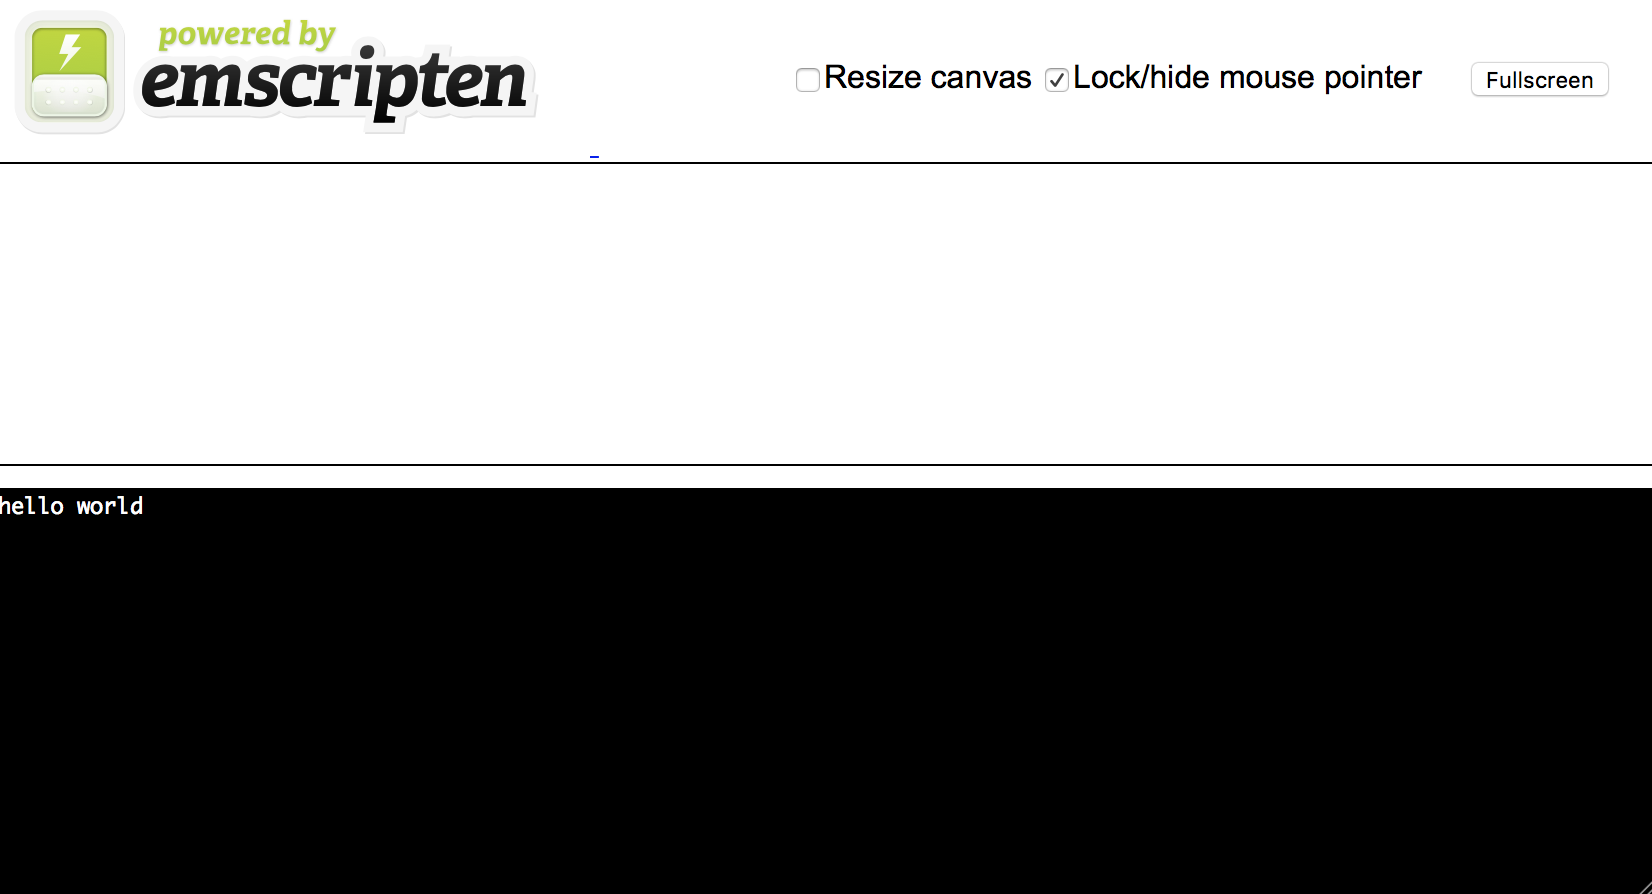
\includegraphics[width=400bp]{figure/pic/hello-world-sample-html.png}
    \caption{hello world移植程序在浏览器中运行效果}
    \label{hello-world-sample-html}
\end{figure}


\section{emscripten编译c/c++文件的原理}

\subsection{emscripten编译c/c++文件的过程}


图\ref{emscripten-compile-step}展示了emscripten编译c/c++文件生成JavaScript文件的过程。

\begin{figure}[h!] % [h!] 表示尽量排在当前位置
    \centering
    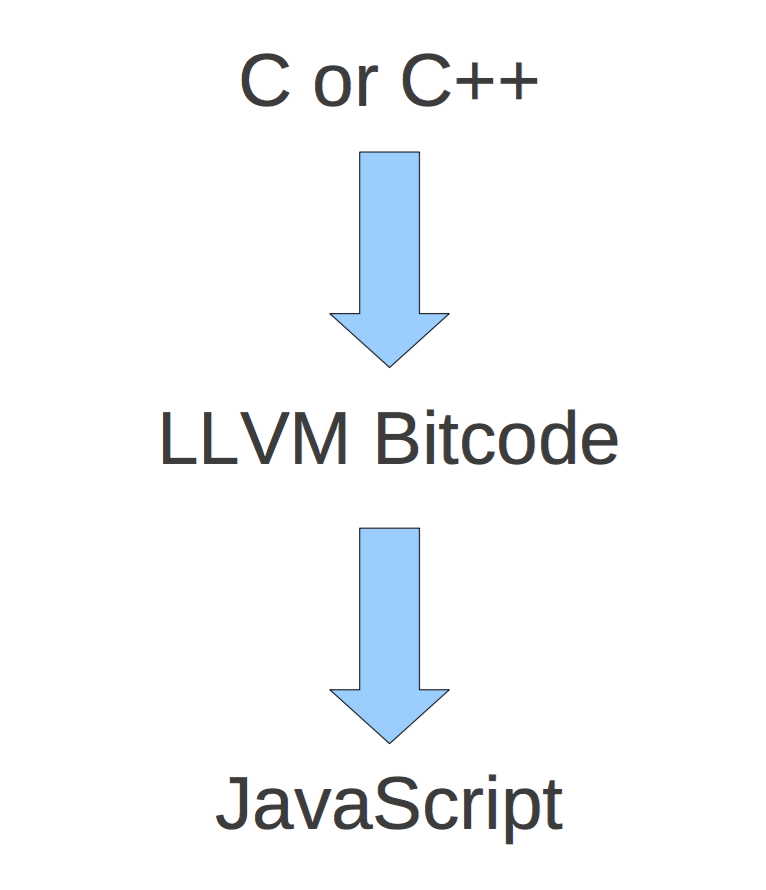
\includegraphics[width=100bp]{figure/pic/emscripten-compile-step.png}
    \caption{emscripten编译c/c++文件的过程}
    \label{emscripten-compile-step}
\end{figure}


依旧以hello world程序为例,hello world源代码如代码\ref{c-hello-world-sample2}所示。

\begin{lstlisting}[
    language={C},
    caption={Hello World程序的源代码},
    label={c-hello-world-sample2},
]
#include <stdio.h>

int main()
{
    printf("Hello, world!");
    return 0;
}
\end{lstlisting}

\newpage

经过clang,编译成llvm字节码,字节码如\ref{c-hello-world-bytecode}所示。

\begin{lstlisting}[
    language={C},
    caption={Hello World程序的llvm字节码},
    label={c-hello-world-bytecode},
]
@.str = private unnamed_addr constant [15 x i8]
             c"hello, world!\0A\00", align 1
define i32 @main() {
entry:
  %retval = alloca i32, align 4
  call i32 (i8*, ...)* @printf(i8* getelementptr
        inbounds ([15 x i8]* @.str, i32 0, i32 0))
  store i32 0, i32* %retval
  ret i32 %retval
}
\end{lstlisting}

该字节码调整一下结构如下\ref{c-hello-world-bytecode2}所示。

\begin{lstlisting}[
    language={C},
    caption={Hello World程序调整后的llvm字节码},
    label={c-hello-world-bytecode2},
]
define i32 @main() {
entry:
  %retval = alloca i32,
            align 4
  call i32 (i8*, ...)*
       @printf (..)
  store i32 0, i32*
        %retval
    ret i32 %retval 
}
\end{lstlisting}

然后由改字节码生成如代码\ref{c-hello-world-gen-js}所示的JavaScript文件。

\begin{lstlisting}[
    language={Java},
    caption={Hello World代码最终生成的js文件},
    label={c-hello-world-gen-js},
]
function _main() {
    var _retval;
    _printf (..);
    _retval = 0;
    return _retval;
}
\end{lstlisting}

\subsection{emscripten编译c/c++文件生成JavaScript文件的原则}

emscripten编译c/c++文件生成JavaScript文件的原则如下所示:

\begin{itemize}[itemindent=2em]
    \item 尽可能 1对1 的进行翻译;
    \item 尽可能把LLVM的内置系统调用替换为JavaScript的内置函数调用;
    \item 尽可能把LLVM变量转换为JavaScript内置变量(而非自定义新的数据结构)。
\end{itemize}

\subsection{emscripten编译生成JavaScript文件的性能分析}

表格\ref{emscripten-performance-sample}展示了emscripten的一个性能测试\upcite{zakai2011emscripten}。
\begin{table}
    \centering
    \caption{emscripten生成代码的执行效率}
    \label{emscripten-performance-sample}
    \begin{tabular}{c|c|c|c|c}
        \hline
        Benchmark & V8 & V8 TA* & SM &SM TA \\ \hline \hline
        dlmalloc & 8.57 & 3.19 & 4.00 & 1.80 \\ \hline
        fannkuch & 78.17 & 2.92 & 6.10 & 4.95 \\ \hline
        fasta & 18.22 & 1.56 & 3.65 & 2.67 \\ \hline
        memops & 239.28 & 4.22 & 6.96 & 6.06 \\ \hline
        primes & 4.64 & 2.16 & 2.59 & 2.48 \\ \hline
        raytrace & 90.40 & 29.28 & 6.03 & 6.80 \\ \hline
    \end{tabular}
\end{table}

\noindent 其中,数字代表生成的js文件运行时长是 gcc 4.6.1 编译同文件得到的的二进制文件运行时长的倍数,
越小越好。

\noindent {\heiti V8} = V8 (Chrome) \\
{\heiti SM} = SpiderMonkey (Firefox) \\ 
{\heiti TA} = Typed Arrays \\
{\heiti *} V8虚拟机并没有类型数组,需要添加一些扩展


通过上面的表格可以得出以下结论:现代JavaScript引擎 (谷歌的V8,Mozilla的SpiderMonkey) 在很多情况下相比原生二进制代码只慢二到三倍(明显快于其他脚本语言)。

但是实际情况下,JavaScript引擎的速度并不能达到那种速度,因为:

\begin{itemize}[itemindent=2em]
    \item Bug;
    \item 不同JavaScript引擎存在差异;
    \item 有些JavaScript引擎的实现不够好;
    \item JavaScript虚拟机运行方式是单线程异步执行,运行针对多线程优化的代码没有优势。
\end{itemize}

\subsection{WebIDL技术}

WebIDL是emscripten的一个重要的第三方工具,由W3C制定。

WebIDL Binder是一个简单轻量的C++绑定方法,通过该方法编译过的C++代码可以在JavaScript中以和普通的JavaScript类库相同的方法调用内部的方法。

WebIDL Binder使用WebIDL\upcite{mccormack2012web}来定义,一种专门用来粘合 C++ 和 JavaScript 的接口定义语言。他是 C++ 类库向 JavaScript 移植的常见选择,而且因为它是面向底层的,它也很容易进行优化。

使用WebIDL Binder来粘合语言需要三步:

\begin{itemize}[itemindent=2em]
    \item 创建一个WebIDL文件来描述C++接口;
    \item 使用Binder生成C++和JavaScript的“胶水”代码;
    \item 将“胶水”代码和工程文件一起,使用Emscripten编译。
\end{itemize}

第一步是创建WebIDL文件来描述你将要粘合的C++类型。这个文件应该会和头文件中的信息重复,这种格式既能简化代码解析,也能简化代码的表示。

举个例子,下面的C++类\ref{c-class-Foo-and-Bar}。

\begin{lstlisting}[
    language={C++},
    caption={Foo和Bar类},
    label={c-class-Foo-and-Bar},
]
class Foo {
public:
  int getVal();
  void setVal(int v);
};

class Bar {
public:
  Bar(long val);
  void doSomething();
};
\end{lstlisting}

\newpage

下面的IDL文件\ref{c-class-Foo-and-Bar-webidl}是用来描述Foo和Bar类的。

\begin{lstlisting}[
    language={C++},
    caption={Foo和Bar类的webidl文件},
    label={c-class-Foo-and-Bar-webidl},
]
interface Foo {
    void Foo();
    long getVal();
    void setVal(long v);
};

interface Bar {
    void Bar(long val);
    void doSomething();
};
\end{lstlisting}

IDL定义和C++源文件之间的映射关系非常明显。需要注意几件事:

\begin{itemize}[itemindent=2em]
    \item IDL类定义包括了一个和接口同名返回值为void的函数。这个构造器可以在JavaScript中直接调用来生成实例,但是必须在IDL中定义,即使C++使用了默认构造器(比如上例中的Foo);
    \item 在WebIDL中使用的类型名不一定和他们在C++中定义时相同(举个例子,上例中int被映射为long)。
\end{itemize}

第二步是生成胶水代码。

粘合剂生成器(bindings generator)(tools/webidl\_binder.py)接收一个WebIDL文件名为输入,输出输入文件的文件名,并创建C++和JavaScript的胶水代码文件。
举个例子,为了使用IDL文件my\_classes.idl生成胶水代码文件glue.cpp和glue.js,需要使用如下的命令\ref{bash-idl-genenrate-glue-files}。

\begin{lstlisting}[
    language={bash},
    caption={使用IDL文件生成胶水代码文件的命令},
    label={bash-idl-genenrate-glue-files},
]
python tools/webidl_binder.py my_classes.idl glue
\end{lstlisting}

接下来是使用胶水代码文件来编译工程。

为了在项目中使用胶水代码文件(glue.cpp和glue.js),需要完成如下工作:

\begin{itemize}[itemindent=2em]
    \item 在编译项目使用的 emcc 命令中添加 \text{--}post\text{-}js glue.js,post\text{-}js参数用来在编译时添加胶水代码;
    \item 创建一个文件,比如my\_glue\_wrapper.cpp,用来\#include你需要粘合的类的头文件以及 glue.cpp 文件,类似代码\ref{add-reference-to-glue-cpp-file}的内容\footnote{由粘合剂生成器(bindings generator)产生的C++胶水代码不包含他们粘合的类的头文件是因为他们无法在WebIDL文件中表示,所以需要创建一个新文件来包含头文件和胶水代码文件。如果不想创建这个新文件,可以把使用到的类的头文件引用添加到glue.cpp的头部,但是每次IDL文件重新编译时该过程都要重来一次};

    \begin{lstlisting}[
        language={C++},
        caption={添加glue.cpp文件的引用},
        label={add-reference-to-glue-cpp-file},
    ]
    #include <...>//"..." represents the headers for the classes we are binding.
    #include <glue.cpp>
    \end{lstlisting}

    \item 在最终的emcc命令中添加my\_glue\_wrapper.cpp文件。

\end{itemize}

最终的emcc文件同时包括C++和JavaScript胶水文件,因为这两者其实一开始就是要一起使用的,可以通过执行代码\ref{bash-add-reference-to-glue-cpp-file}来实现。
\begin{lstlisting}[
    language={C++},
    caption={编译时添加胶水文件修饰},
    label={bash-add-reference-to-glue-cpp-file},
]
./emcc my_classes.cpp my_glue_wrapper.cpp --post-js glue.js -o output.js
\end{lstlisting}

现在,输出的js文件中可以直接创建C++中定义的实例。

当绑定完成后,引入之前生成的js文件,可以直接实例化Foo对象和Bar对象,和实例化JavaScript对象的方法完全相同,就好像Foo和Bar对象本身就是JavaScript原生对象。继续上面的例子,你可以创建Foo和Bar对象的实例并调用他们的内部方法,如代码\ref{create-c-class-in-js-file}所示。


\begin{lstlisting}[
    language={Java},
    caption={在JavaScript中生成Foo和Bar实例},
    label={create-c-class-in-js-file},
]
var f = new Module.Foo();
f.setVal(200);
alert(f.getVal());

var b = new Module.Bar(123);
b.doSomething();
\end{lstlisting}

使用Module对象来获取对象 虽然一般情况下对象在全局命令空间,但也存在例外(比如你使用closure编译器\upcite{livshits2015defense}来压缩和包装编译后的代码来避免污染全局命名空间)。你也可以修改Module的名字,比如使用var MyModuleName = Module;可以把Module的名字修改为MyModuleName。

JavaScript有自动垃圾回收功能,在包装的C++对象不再被使用后,会启用gc。如果C++对象不需要特别指明被清理(甚至没有析构函数),你什么都不用做。

如果一个C++对象确实需要被清理,你需要明确调用Module.destroy(obj)来调用析构函数,然后删除所有引用对象,以便它可以被垃圾收集。举个例子,如果要手动清除Bar被分配的内存,可使用如下代码\ref{js-module-gc-by-hand}所示的方法。

\begin{lstlisting}[
    language={Java},
    caption={在JavaScript中手动清理module内存},
    label={js-module-gc-by-hand},
]
var b = new Module.Bar(123);
b.doSomething();
Module.destroy(b); // If the C++ object requires clean up
\end{lstlisting}

当在JavaScript中创建C++对象时,需要显示调用C++构造器。但是没有办法得知某个JavaScript对象要被垃圾回收,所以胶水语言不能自动调用析构函数 。
通常你需要销毁你自己创建的对象,取决于你移植的类库。

需要注意的是,WebIDL中的类型名使用的关键字和C++类型名关键字不完全相同,以下表\ref{webidl-types-from-c-types}是一些在WebIDL和C++中常见类型的对应关系表。

\begin{table}
    \centering
    \caption{webIDL和C++类型映射}
    \label{webidl-types-from-c-types}
    \begin{tabular}{c|c}
        \hline
        C++ & IDL  \\ \hline \hline
        bool  &  boolean \\ \hline
        float &  float  \\ \hline
        double &  double  \\ \hline
        char &   byte  \\ \hline
        char* &  DOMString (represents a JavaScript string)  \\ \hline
        unsigned char &  octet  \\ \hline
        unsigned short int & unsigned short  \\ \hline
        unsigned short & unsigned short  \\ \hline
        unsigned long  & unsigned long  \\ \hline
        int & long  \\ \hline
        void  &  void  \\ \hline
        void* &  any or VoidPtr (see void*)  \\ \hline
    \end{tabular}
\end{table}









